\documentclass[11pt]{article}
\usepackage[margin=1in]{geometry}
\usepackage{graphicx}
\usepackage{booktabs}
\title{PC--Atomic Properties Note (AtomicProps Extension)}
\date{}
\begin{document}
\maketitle

\section*{Data used}
\begin{itemize}
\item Features: \texttt{2026-02-16/artifacts/2026-02-16/reports/bandcount/K\_37/features.csv}
\item External atomic properties: \texttt{data/external/atomic\_properties/atomic\_properties\_clean.csv}
\item Merged analysis table: \texttt{reports/elements\_pcs\_atomicprops\_merged.csv}
\end{itemize}

\section*{Preprocessing}
Columns of the 37-band matrix were z-scored, PCA was computed from the correlation matrix, and PC scores were merged with cleaned atomic properties by atomic number.

\section*{Key correlation outputs}
See JSON outputs:
\begin{itemize}
\item \texttt{reports/pc\_atomicprops\_correlations.json}
\item \texttt{reports/pc\_atomicprops\_partial\_correlations.json}
\item \texttt{reports/pc\_atomicprops\_permutation\_pvalues.json}
\end{itemize}

\section*{Permutation summary}
Two-sided permutation tests (1000 shuffles) were computed for key PC1 relationships: period, first ionization energy, electronegativity, and atomic radius.

\section*{Cautious interpretation}
These results quantify associations between latent spectral PCs and atomic descriptors in the current dataset. They are descriptive and sensitive to feature construction, missingness handling, and merge coverage.

\section*{Figures}
\begin{figure}[h!]
\centering
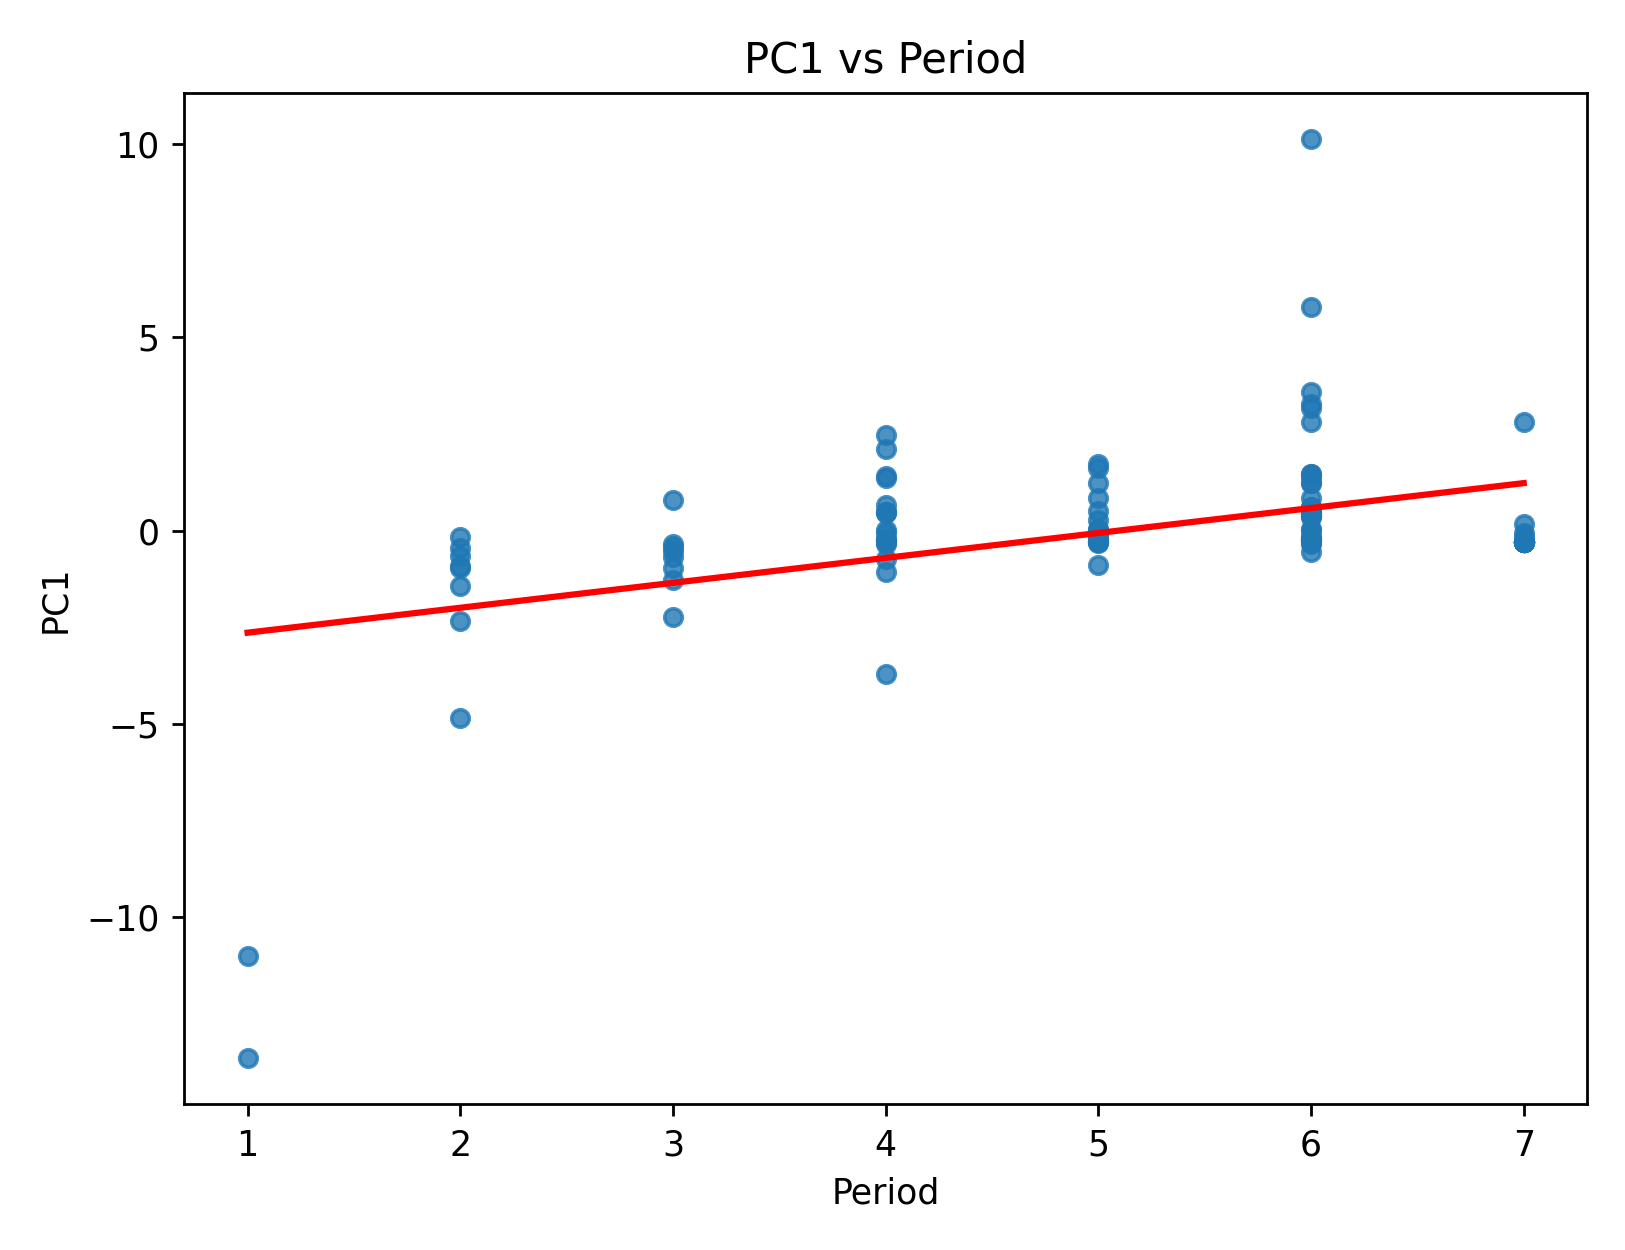
\includegraphics[width=0.65\textwidth]{figures/fig_pc1_vs_period.png}
\caption{PC1 vs period.}
\end{figure}

\begin{figure}[h!]
\centering
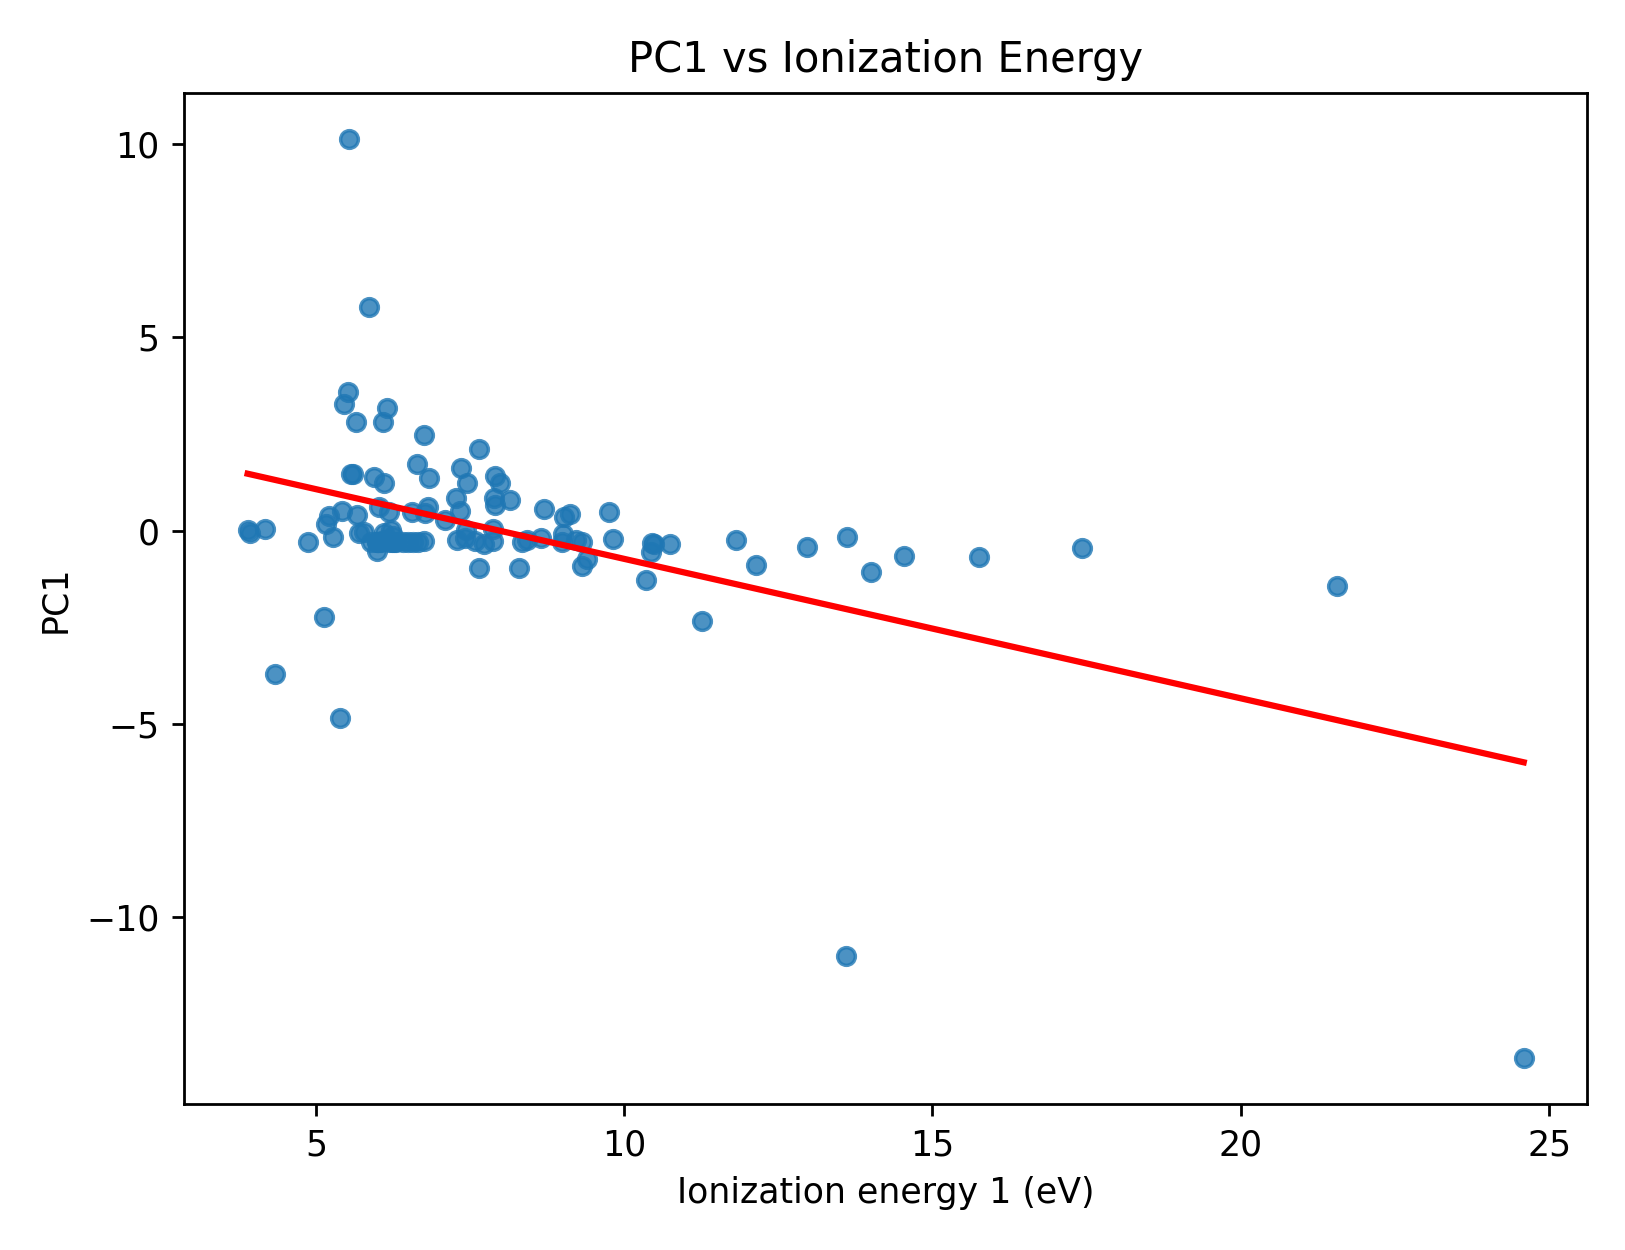
\includegraphics[width=0.65\textwidth]{figures/fig_pc1_vs_ionization.png}
\caption{PC1 vs first ionization energy.}
\end{figure}

\begin{figure}[h!]
\centering
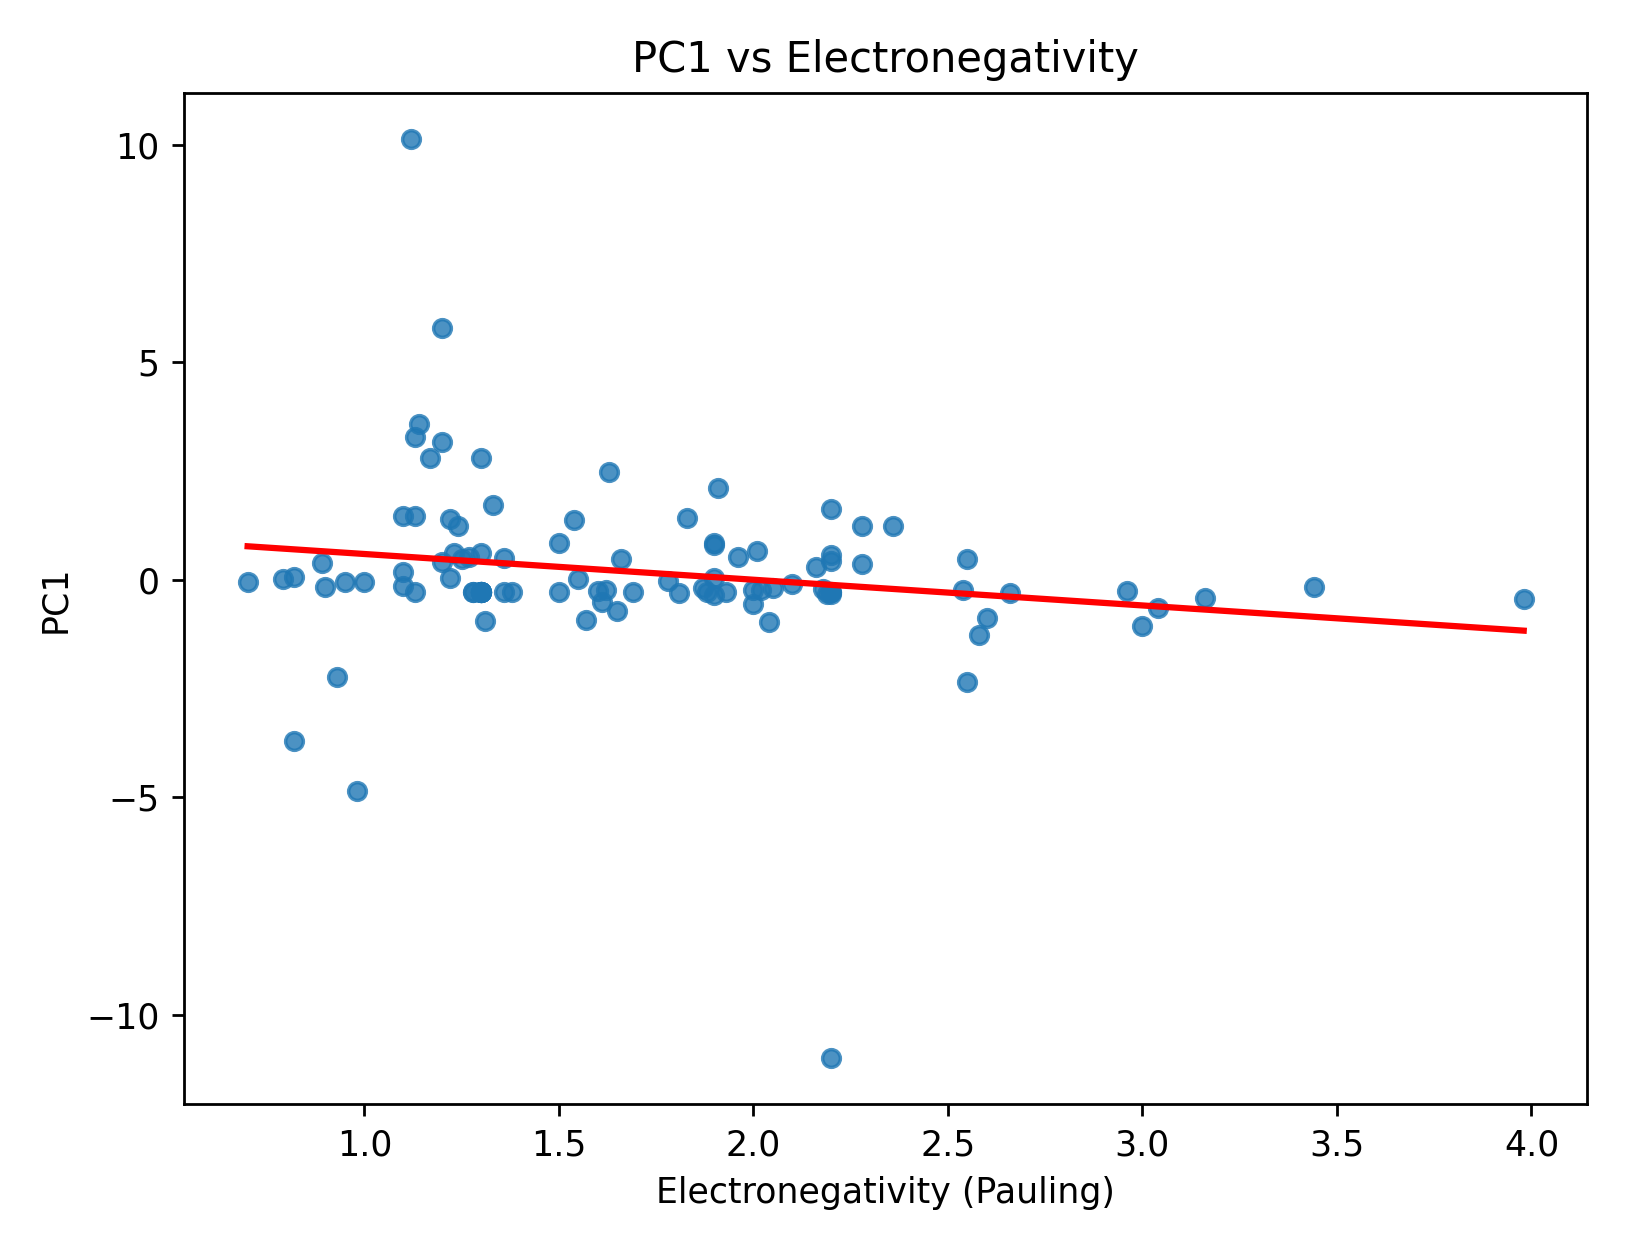
\includegraphics[width=0.65\textwidth]{figures/fig_pc1_vs_electronegativity.png}
\caption{PC1 vs electronegativity.}
\end{figure}

\begin{figure}[h!]
\centering
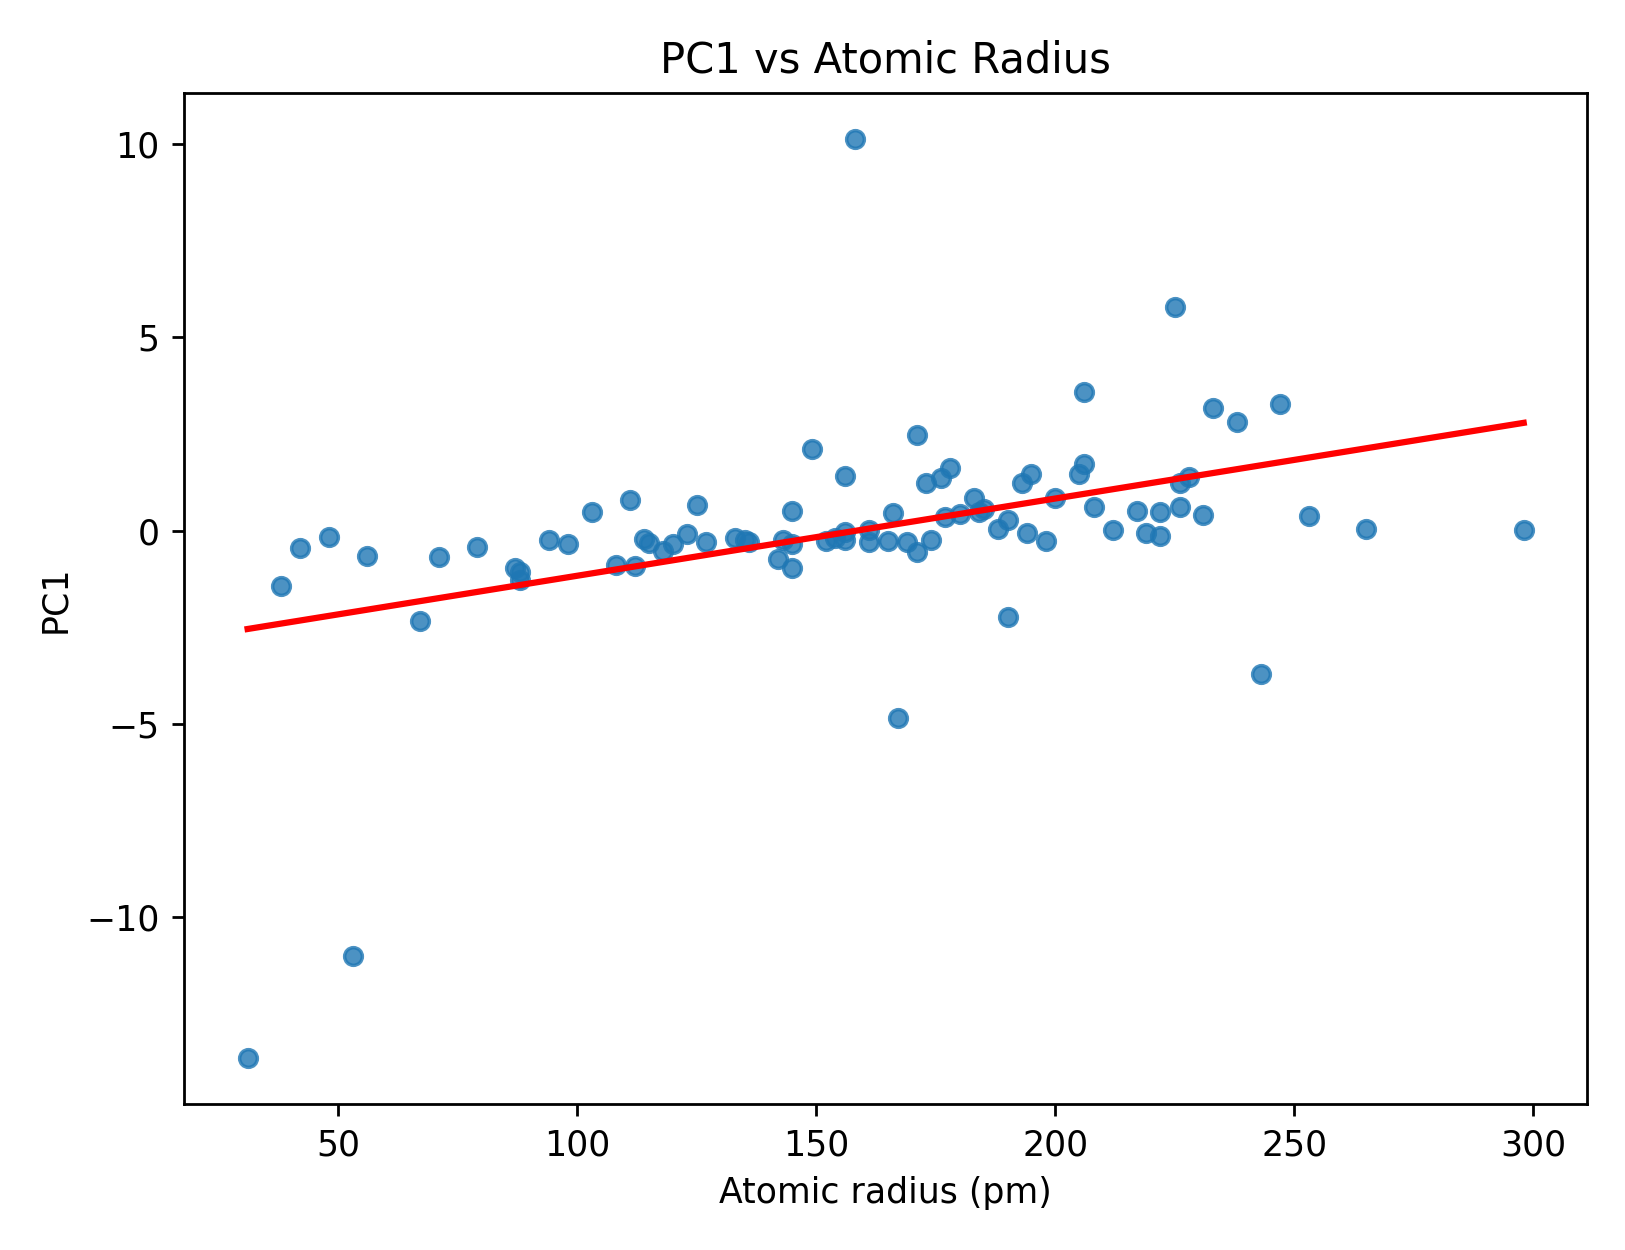
\includegraphics[width=0.65\textwidth]{figures/fig_pc1_vs_radius.png}
\caption{PC1 vs atomic radius.}
\end{figure}

\begin{figure}[h!]
\centering
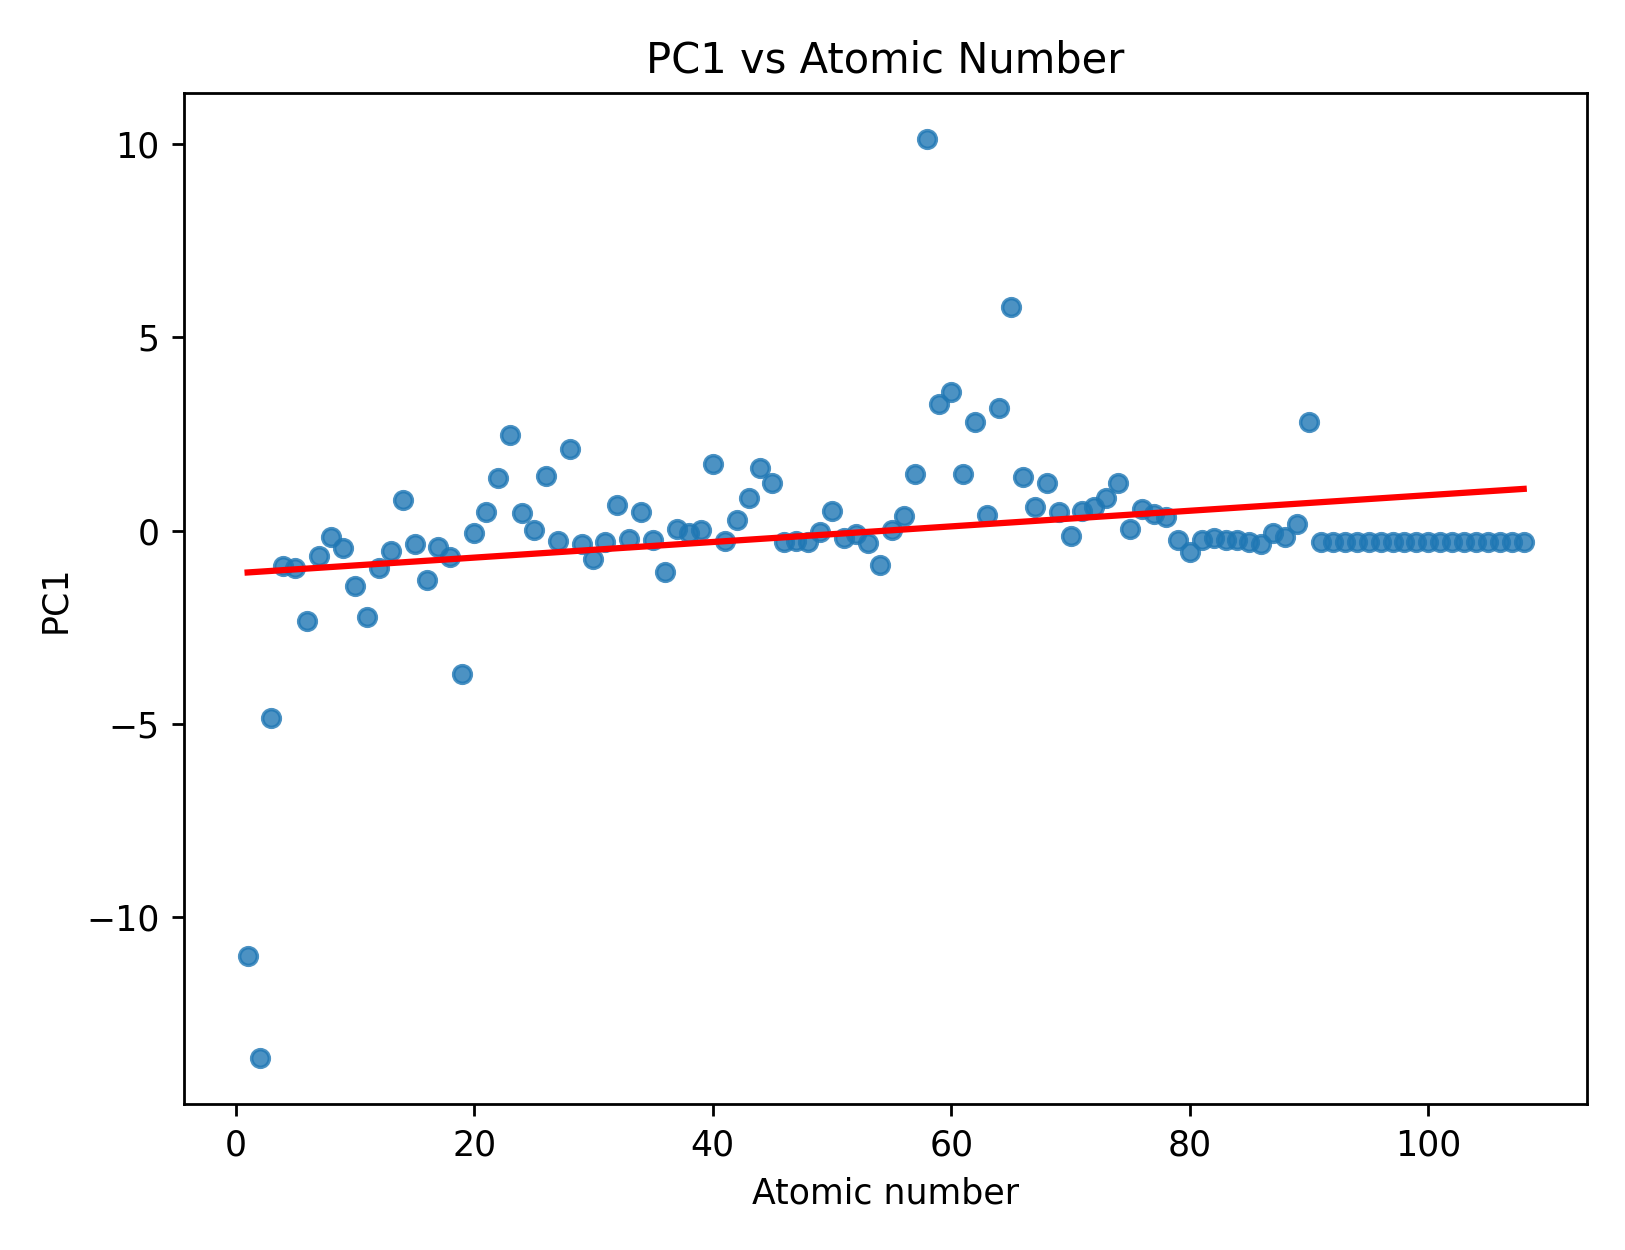
\includegraphics[width=0.65\textwidth]{figures/fig_pc1_vs_atomic_number.png}
\caption{PC1 vs atomic number.}
\end{figure}

\end{document}
